% Options for packages loaded elsewhere
\PassOptionsToPackage{unicode}{hyperref}
\PassOptionsToPackage{hyphens}{url}
\PassOptionsToPackage{dvipsnames,svgnames,x11names}{xcolor}
%
\documentclass[
  letterpaper,
  DIV=11,
  numbers=noendperiod]{scrreprt}

\usepackage{amsmath,amssymb}
\usepackage{lmodern}
\usepackage{iftex}
\ifPDFTeX
  \usepackage[T1]{fontenc}
  \usepackage[utf8]{inputenc}
  \usepackage{textcomp} % provide euro and other symbols
\else % if luatex or xetex
  \usepackage{unicode-math}
  \defaultfontfeatures{Scale=MatchLowercase}
  \defaultfontfeatures[\rmfamily]{Ligatures=TeX,Scale=1}
\fi
% Use upquote if available, for straight quotes in verbatim environments
\IfFileExists{upquote.sty}{\usepackage{upquote}}{}
\IfFileExists{microtype.sty}{% use microtype if available
  \usepackage[]{microtype}
  \UseMicrotypeSet[protrusion]{basicmath} % disable protrusion for tt fonts
}{}
\makeatletter
\@ifundefined{KOMAClassName}{% if non-KOMA class
  \IfFileExists{parskip.sty}{%
    \usepackage{parskip}
  }{% else
    \setlength{\parindent}{0pt}
    \setlength{\parskip}{6pt plus 2pt minus 1pt}}
}{% if KOMA class
  \KOMAoptions{parskip=half}}
\makeatother
\usepackage{xcolor}
\setlength{\emergencystretch}{3em} % prevent overfull lines
\setcounter{secnumdepth}{5}
% Make \paragraph and \subparagraph free-standing
\ifx\paragraph\undefined\else
  \let\oldparagraph\paragraph
  \renewcommand{\paragraph}[1]{\oldparagraph{#1}\mbox{}}
\fi
\ifx\subparagraph\undefined\else
  \let\oldsubparagraph\subparagraph
  \renewcommand{\subparagraph}[1]{\oldsubparagraph{#1}\mbox{}}
\fi


\providecommand{\tightlist}{%
  \setlength{\itemsep}{0pt}\setlength{\parskip}{0pt}}\usepackage{longtable,booktabs,array}
\usepackage{calc} % for calculating minipage widths
% Correct order of tables after \paragraph or \subparagraph
\usepackage{etoolbox}
\makeatletter
\patchcmd\longtable{\par}{\if@noskipsec\mbox{}\fi\par}{}{}
\makeatother
% Allow footnotes in longtable head/foot
\IfFileExists{footnotehyper.sty}{\usepackage{footnotehyper}}{\usepackage{footnote}}
\makesavenoteenv{longtable}
\usepackage{graphicx}
\makeatletter
\def\maxwidth{\ifdim\Gin@nat@width>\linewidth\linewidth\else\Gin@nat@width\fi}
\def\maxheight{\ifdim\Gin@nat@height>\textheight\textheight\else\Gin@nat@height\fi}
\makeatother
% Scale images if necessary, so that they will not overflow the page
% margins by default, and it is still possible to overwrite the defaults
% using explicit options in \includegraphics[width, height, ...]{}
\setkeys{Gin}{width=\maxwidth,height=\maxheight,keepaspectratio}
% Set default figure placement to htbp
\makeatletter
\def\fps@figure{htbp}
\makeatother
\newlength{\cslhangindent}
\setlength{\cslhangindent}{1.5em}
\newlength{\csllabelwidth}
\setlength{\csllabelwidth}{3em}
\newlength{\cslentryspacingunit} % times entry-spacing
\setlength{\cslentryspacingunit}{\parskip}
\newenvironment{CSLReferences}[2] % #1 hanging-ident, #2 entry spacing
 {% don't indent paragraphs
  \setlength{\parindent}{0pt}
  % turn on hanging indent if param 1 is 1
  \ifodd #1
  \let\oldpar\par
  \def\par{\hangindent=\cslhangindent\oldpar}
  \fi
  % set entry spacing
  \setlength{\parskip}{#2\cslentryspacingunit}
 }%
 {}
\usepackage{calc}
\newcommand{\CSLBlock}[1]{#1\hfill\break}
\newcommand{\CSLLeftMargin}[1]{\parbox[t]{\csllabelwidth}{#1}}
\newcommand{\CSLRightInline}[1]{\parbox[t]{\linewidth - \csllabelwidth}{#1}\break}
\newcommand{\CSLIndent}[1]{\hspace{\cslhangindent}#1}

\KOMAoption{captions}{tableheading}
\makeatletter
\makeatother
\makeatletter
\@ifpackageloaded{bookmark}{}{\usepackage{bookmark}}
\makeatother
\makeatletter
\@ifpackageloaded{caption}{}{\usepackage{caption}}
\AtBeginDocument{%
\ifdefined\contentsname
  \renewcommand*\contentsname{Table of contents}
\else
  \newcommand\contentsname{Table of contents}
\fi
\ifdefined\listfigurename
  \renewcommand*\listfigurename{List of Figures}
\else
  \newcommand\listfigurename{List of Figures}
\fi
\ifdefined\listtablename
  \renewcommand*\listtablename{List of Tables}
\else
  \newcommand\listtablename{List of Tables}
\fi
\ifdefined\figurename
  \renewcommand*\figurename{Figure}
\else
  \newcommand\figurename{Figure}
\fi
\ifdefined\tablename
  \renewcommand*\tablename{Table}
\else
  \newcommand\tablename{Table}
\fi
}
\@ifpackageloaded{float}{}{\usepackage{float}}
\floatstyle{ruled}
\@ifundefined{c@chapter}{\newfloat{codelisting}{h}{lop}}{\newfloat{codelisting}{h}{lop}[chapter]}
\floatname{codelisting}{Listing}
\newcommand*\listoflistings{\listof{codelisting}{List of Listings}}
\makeatother
\makeatletter
\@ifpackageloaded{caption}{}{\usepackage{caption}}
\@ifpackageloaded{subcaption}{}{\usepackage{subcaption}}
\makeatother
\makeatletter
\@ifpackageloaded{tcolorbox}{}{\usepackage[many]{tcolorbox}}
\makeatother
\makeatletter
\@ifundefined{shadecolor}{\definecolor{shadecolor}{rgb}{.97, .97, .97}}
\makeatother
\makeatletter
\makeatother
\ifLuaTeX
  \usepackage{selnolig}  % disable illegal ligatures
\fi
\IfFileExists{bookmark.sty}{\usepackage{bookmark}}{\usepackage{hyperref}}
\IfFileExists{xurl.sty}{\usepackage{xurl}}{} % add URL line breaks if available
\urlstyle{same} % disable monospaced font for URLs
\hypersetup{
  pdftitle={Schmidt Ocean Institute Technical Documentation},
  pdfauthor={Schmidt Ocean Institute},
  colorlinks=true,
  linkcolor={blue},
  filecolor={Maroon},
  citecolor={Blue},
  urlcolor={Blue},
  pdfcreator={LaTeX via pandoc}}

\title{Schmidt Ocean Institute Technical Documentation}
\author{Schmidt Ocean Institute}
\date{5/22/23}

\begin{document}
\maketitle
\ifdefined\Shaded\renewenvironment{Shaded}{\begin{tcolorbox}[frame hidden, borderline west={3pt}{0pt}{shadecolor}, enhanced, interior hidden, sharp corners, boxrule=0pt, breakable]}{\end{tcolorbox}}\fi

\renewcommand*\contentsname{Table of contents}
{
\hypersetup{linkcolor=}
\setcounter{tocdepth}{2}
\tableofcontents
}
\bookmarksetup{startatroot}

\hypertarget{preface}{%
\chapter*{Preface}\label{preface}}
\addcontentsline{toc}{chapter}{Preface}

\markboth{Preface}{Preface}

Schmidt Ocean Insititute

Public technical documentation related to data systems.

\bookmarksetup{startatroot}

\hypertarget{introduction}{%
\chapter{Introduction}\label{introduction}}

This will be a book that contains chapters on accessing data systems
while onboard R/V Falkor (too)

\bookmarksetup{startatroot}

\hypertarget{cruise-data-directory-structure}{%
\chapter{Cruise Data Directory
Structure}\label{cruise-data-directory-structure}}

\bookmarksetup{startatroot}

\hypertarget{dashboards}{%
\chapter{Dashboards}\label{dashboards}}

\bookmarksetup{startatroot}

\hypertarget{sealog-subastian-configuration-and-use}{%
\chapter{Sealog-Subastian Configuration and
Use}\label{sealog-subastian-configuration-and-use}}

R/V Falkor (too)

\hypertarget{overview}{%
\section{Overview}\label{overview}}

Sealog SuBastian is a smart event logger for ROV SuBastian dives that
couples key metadata (such as video framegrabs, vehicle position,
vehicle depth, water temperature, etc.) with each event. Sealog can be
configured for each cruise to better support a science party's specific
data logging needs. After each dive, Sealog creates an extensive ``Dive
Summary PDF'' with all the events recorded during the dive, along with
other useful graphics.

\hypertarget{orientation}{%
\section{Orientation}\label{orientation}}

Sealog can be found either at 10.23.11.25/sealog-Sub/ in any web
browser, or you can use the ``Sealog-Subastian'' link at 10.23.11.25.
Currently, Sealog can only be reached while onboard the ship.

\hypertarget{login}{%
\section{Login}\label{login}}

We recommend that each science party member create their own individual
login for Sealog. With each event entry, along with the scientific
metadata, the system will keep track of the user that submitted the
entry. There is also a guest login that has access to creating events,
but has restricted access to event template configurations.

\begin{figure}

\begin{minipage}[t]{0.50\linewidth}

{\centering 

\raisebox{-\height}{

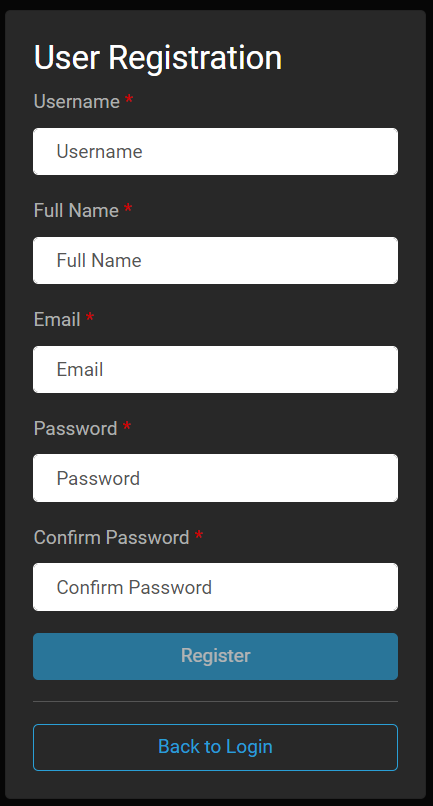
\includegraphics{././images/image22.png}

}

}

\end{minipage}%
%
\begin{minipage}[t]{0.50\linewidth}

{\centering 

\raisebox{-\height}{

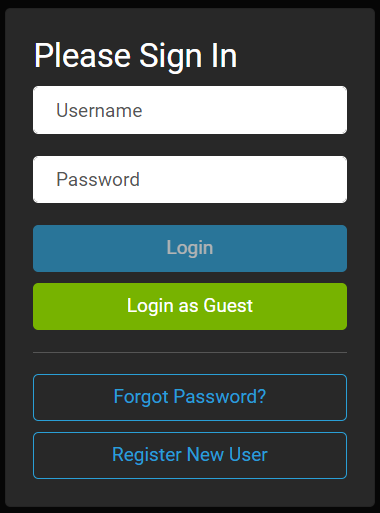
\includegraphics{././images/image19.png}

}

}

\end{minipage}%

\end{figure}

\hypertarget{templates}{%
\section{Templates}\label{templates}}

System templates are event configurations that are logged and maintained
by the ship's crew to monitor key milestones during each dive (ex. in
water/out of water times, on/off bottom times, video start/stop). These
events are admin access only and cannot be edited by the science party.
Event templates can be edited by the science party and are meant to be
tailored to meet the science parties' data logging needs.

\hypertarget{event-template-configuration}{%
\subsection{Event Template
Configuration}\label{event-template-configuration}}

This section will orient you on how to create Sealog ``events.'' It is
important to note that the primary way of accessing exported data is via
a spreadsheet. All ``Event Values'' and ``Event Option'' names should be
concise.

\hypertarget{adding-an-event-template}{%
\subsubsection{Adding an Event
Template}\label{adding-an-event-template}}

\begin{itemize}
\tightlist
\item
  Once logged in, navigate to ``System Management'' then select ``Event
  Management.''

  \begin{itemize}
  \tightlist
  \item
    Please note you need to be logged in as a user, ``Guest'' does not
    have event management access.
  \end{itemize}
\end{itemize}

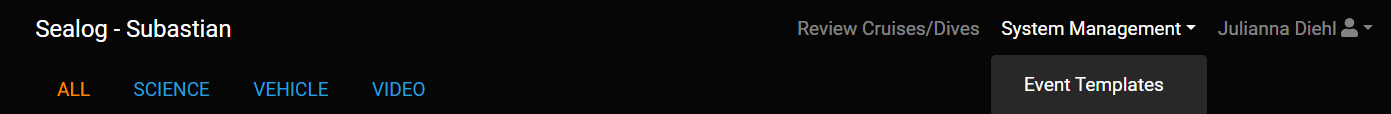
\includegraphics{images/image21.png}

\begin{itemize}
\tightlist
\item
  On the right hand side, the open for ``Create Event Template'' will
  allow you to create a new event.
\end{itemize}

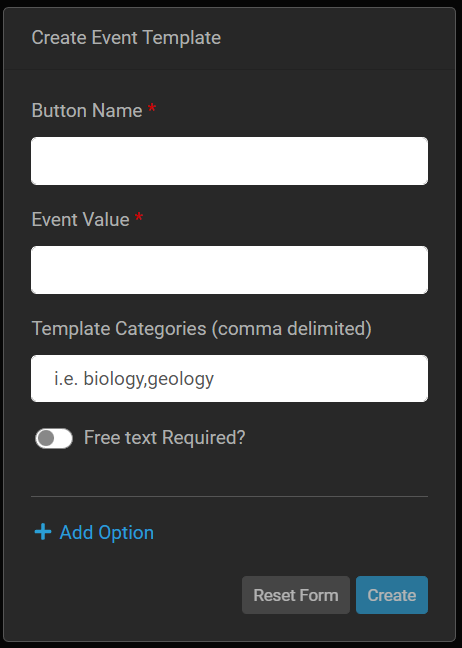
\includegraphics[width=0.4\textwidth,height=\textheight]{images/image9.png}

\hypertarget{button-name}{%
\subsubsection{Button Name}\label{button-name}}

Button name is the title of the event. In the example below, the button
name is ``Video Logging'' and is used by the SuBastian team to log when
the DVR's begin recording.

\hypertarget{event-value}{%
\subsubsection{Event Value}\label{event-value}}

Event values are a way of grouping events. For example, if you have
several events that count as sampling (ex. coral collection, niskin
sampling, biological sampling, etc.,) they can all be grouped as the
event value ``Sample.'' In the dive summary pdf that gets created at the
end of every dive, each Event Value will have its own section,
summarizing all of the events under the particular Event Value for that
dive.

The screenshot below shows an example of events that were labeled with
the Event Value ``Sample'' and the different types denote whether they
are biological, niskins, or squeezer samples in this dive.

\hypertarget{template-categories}{%
\subsubsection{Template Categories}\label{template-categories}}

Template Categories create different tabs in the home screen to further
organize event buttons. In the example below, there are three template
categories configured: science, vehicle, video. By default, the ``All''
category will always show every event button configured.

\includegraphics{images/temp.png}

Some science parties may want to broaden their own Template Categories
beyond the single ``Science'' that is the default configuration, ex.
``Observation, Sample, etc.'' The ``Vehicle'' and ``Video'' template
categories contain important vehicle milestones and should be left
unchanged.

\hypertarget{free-text-event}{%
\subsubsection{Free Text Event}\label{free-text-event}}

It is also possible to enter ``free text events''. These are events that
are logged without using event templates. This could be useful for quick
notes, corrections, or if there is not a current event template
configured for a certain situation during a dive.

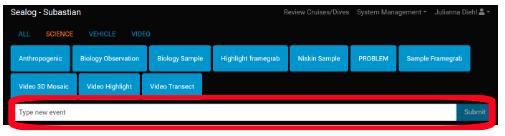
\includegraphics{images/freetext.png}

\hypertarget{configuring-event-options}{%
\subsubsection{Configuring Event
Options}\label{configuring-event-options}}

At the bottom of the ``Create Event Template'' the ``+ Add Option''
selection gives you further options to tailor each event.

\hypertarget{name}{%
\paragraph{Name}\label{name}}

The name of the event option describes the specific option you are
creating. For example, in the screenshot below, there are two options
configured. The first option, named ``Action'' allows you to choose to
either start or stop the dive stream radio buttons. The second option,
named ``Platform'' allows you to choose checkboxes for the platforms
that are being started.

\begin{itemize}
\tightlist
\item
  Event options cannot be named ``id'' or ``comment''- these are
  reserved keywords.
\end{itemize}

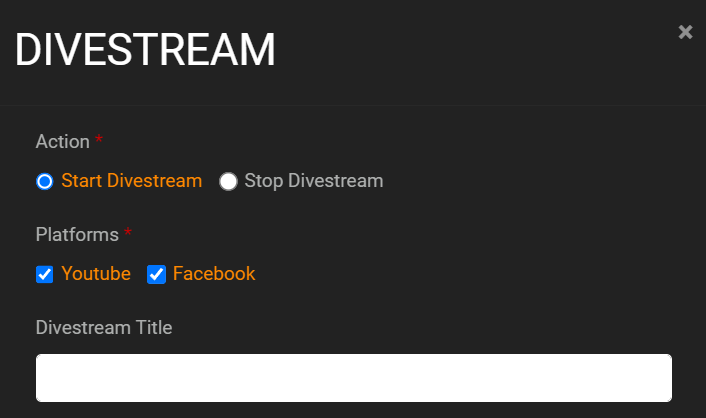
\includegraphics[width=0.4\textwidth,height=\textheight]{images/image8.png}

\hypertarget{type}{%
\paragraph{Type}\label{type}}

The type describes the choice of action you have for this option. The
options are described in more detail below.

\begin{itemize}
\item
  Static Text

  Static text options are for when the value is known and should not be
  altered. This can be used when the act of clicking the event button is
  all that is needed to log the event. In the example below, the event
  ``Vehicle on Deck'' will always have a value of ``On Deck.''

  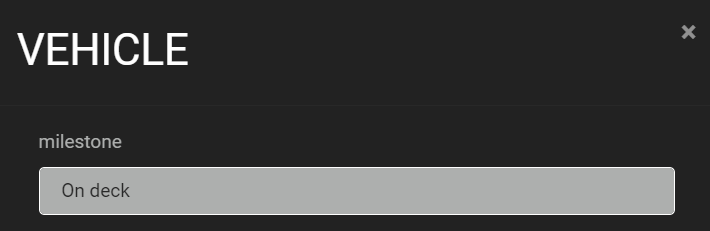
\includegraphics[width=0.4\textwidth,height=\textheight]{images/image15.png}
\item
  Text

  The text option is for when the value possibilities for the option are
  unknown and must be manually filled out when the event is submitted.
  This could be used when describing file names, writing the species
  name of an animal observed during a dive, describing a frame grab, and
  more.

  
\includegraphics[width=0.4\textwidth,height=\textheight]{images/image10.png}
\item
  Dropdown

  The dropdown option is for when the option is one out of a long list
  of possibilities. In the example below, a dropdown is used to describe
  all of the octocoral species to aid in a biological observation event.

  \includegraphics[width=0.4\textwidth,height=\textheight]{images/dropdown.png}
\item
  Checkboxes

  Checkboxes are for when the option is one or more of a list of
  possibilities. In the example below, this event allows the user to say
  they're starting both Facebook and YouTube streams, or just one.

  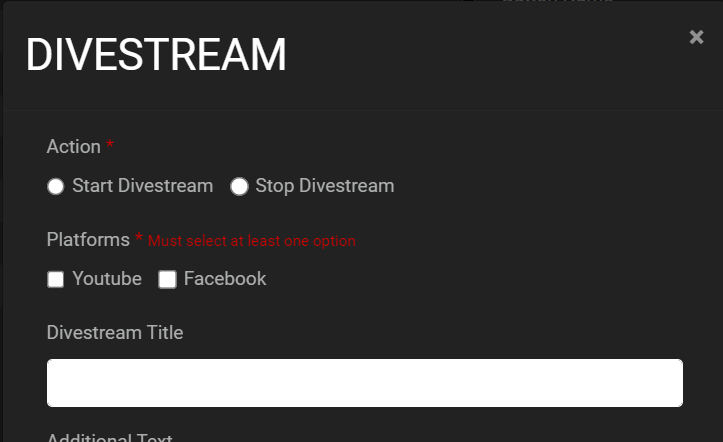
\includegraphics[width=0.4\textwidth,height=\textheight]{images/image23.png}
\item
  Radio Buttons

  Radio buttons are for when the option is one of a short list of
  possibilities. In the option below, the radio buttons are used to
  describe an action of starting or stopping the divestream, while
  checkboxes are used to choose one or all of the listed platforms.

  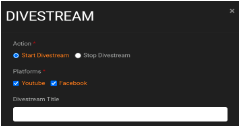
\includegraphics[width=0.4\textwidth,height=\textheight]{images/radio.png}
\item
  Required Button

  The required button allows you to choose if an entry is necessary
  before the event can be created. For example, you may want to have any
  entry that requires a Sample ID or file name as ``required'' so this
  can't accidentally be reported without key information.

  
\includegraphics[width=0.4\textwidth,height=\textheight]{images/image7.png}
\item
  Additional Text

  Default with every Event Template, an additional text box will be
  added that can be used to document any extra information.
\end{itemize}

\hypertarget{saving-and-testing-events}{%
\subsection{Saving and Testing Events}\label{saving-and-testing-events}}

\begin{itemize}
\tightlist
\item
  Click ``Create'' to save your event to the ``Event Templates.''
\item
  
\includegraphics{images/image4.png} Click to edit an Event Template.
\item
  
\includegraphics{images/image35.png} Click to test an Event Template.
  This is useful when making new events to make sure all your options
  are configured how you mean them to be.
\item
  
\includegraphics{images/image26.png}Click to delete an Event Template.
  Please ask an MT if you need to delete an event template that was not
  created by your science party.
\end{itemize}

\hypertarget{samples}{%
\section{Samples}\label{samples}}

Please follow the following requirements for logging your sample's on
Sealog to ensure they will be properly calculated in Sealog's post-dive
metrics. Please note that in all events that have the word ``sample'' in
the ``Event Value'' will be used towards the total number of samples.
For sample events, the ``Event Value'' should ALWAYS be ``SAMPLE'' and
should be configured with the following options:

\begin{itemize}
\item
  Type

  to specify the type of sample collected i.e.~``biology, geology, eDNA,
  Niskin, etc''. This should be configured as a required option. If the
  desire is to have a dedicated button for a specific sample type then
  set this option as ``static text'' with the ``value'' set to the
  sample type i.e.~``eDNA''. If the event template is for multiple
  sample types then the ``Type'' option should have an option type of
  ``dropdown'' or ``radio buttons''.
\item
  Sample ID

  to define the sample's unique identification. This generally will be a
  ``text'' option. This should also be configured as a required option.
\item
  Storage Location

  the unique location on the vehicle where the sample is stored. This
  should be configured as a required option. This option should have an
  option type of ``dropdown'' or ``radio buttons.'' Refer to the list of
  standard vehicle locations (below) for how to populate the event
  option values. If the sample is collected with a science-supplied
  sampling apparatus then the option value should be a list of unique
  identifications for the apparatus type. Ensure that the naming
  convention used for any science-supplied sampling apparatus does not
  conflict with the standard location names.
\end{itemize}

\begin{longtable}[]{@{}ll@{}}
\caption{SuBastian Standard Sample Storage Locations}\tabularnewline
\toprule()
Full Name & ID \\
\midrule()
\endfirsthead
\toprule()
Full Name & ID \\
\midrule()
\endhead
Bio-Box 1A & BB-1A \\
Bio-Box 1B & BB-1B \\
Bio-Box 2A & BB-2A \\
Bio-Box 2B & BB-2B \\
Bio-Box 3A & BB-3A \\
Bio-Box 3B & BB-3B \\
Bottle 01 & BTL-1 \\
Bottle 02 & BTL-2 \\
Bottle 03 & BTL-3 \\
Bottle 04 & BTL-4 \\
Bottle 05 & BTL-5 \\
Bottle 06 & BTL-6 \\
Quiver 01 & Q-1 \\
Quiver 02 & Q-2 \\
Quiver 03 & Q-3 \\
Quiver 04 & Q-4 \\
Quiver 05 & Q-5 \\
Quiver 06 & Q-6 \\
Quiver 07 & Q-7 \\
Quiver 08 & Q-8 \\
Quiver 09 & Q-9 \\
Quiver 10 & Q-10 \\
Quiver 11 & Q-11 \\
Quiver 12 & Q-12 \\
Quiver 13 & Q-13 \\
Quiver 14 & Q-14 \\
Quiver 15 & Q-15 \\
Quiver 16 & Q-16 \\
Suction 01 & S-1 \\
Suction 02 & S-2 \\
Suction 03 & S-4 \\
Suction 04 & S-4 \\
Suction 05 & S-5 \\
Suction 06 & S-6 \\
Suction 07 & S-7 \\
Suction 08 & S-8 \\
\bottomrule()
\end{longtable}

\hypertarget{metadata}{%
\section{Metadata}\label{metadata}}

With each event logged, the following metadata gets grabbed with it:

\hypertarget{rov-video-frame-grabs}{%
\subsubsection{ROV Video Frame Grabs}\label{rov-video-frame-grabs}}

\begin{verbatim}
High resolution screen capture on all cameras.
\end{verbatim}

\begin{itemize}
\tightlist
\item
  Science Camera (4K camera)
\item
  Situation Camera (4K camera)
\item
  HD Quad

  \begin{itemize}
  \tightlist
  \item
    Forward HD Cam, looking to Port.
  \item
    Aft HD Cam, looking Aft.
  \item
    Forward HD Cam, looking down onto the Porch.
  \item
    Forward HD Cam, looking to Stbd.
  \end{itemize}
\item
  SD Quad

  \begin{itemize}
  \tightlist
  \item
    SD Teather Cam, looking aft
  \item
    SD Manifold Cam
  \item
    Suction Sampler Cam
  \item
    Port Manipulator Cam
  \end{itemize}
\end{itemize}

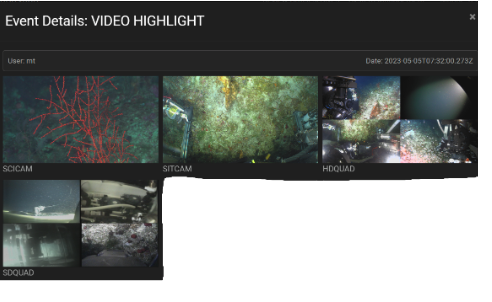
\includegraphics{images/eventdetails.png}

\hypertarget{vessel-realtime-nav-data}{%
\subsubsection{Vessel Realtime Nav
Data}\label{vessel-realtime-nav-data}}

\begin{itemize}
\tightlist
\item
  Falkor (too) position and true heading.
\end{itemize}

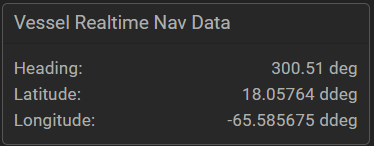
\includegraphics{images/image2.png}

\hypertarget{vehicle-realtime-nav-data}{%
\subsection{Vehicle Realtime Nav Data}\label{vehicle-realtime-nav-data}}

\begin{itemize}
\tightlist
\item
  SuBastian position as calculated by its Sprint Inertial Navigation
  System, which takes several aiding sensors (Ultra Short BaseLine
  underwater positioning system, Doppler Velocity Log sensors, depth
  sensors) along with its own internal inertial sensors and
  accelerometers and uses an algorithm to output the most accurate
  position based on weighted sensor inputs.
\item
  This is generally the most accurate position for the ROV, but it's
  important to confirm this with the Marine Technicians during the
  cruise.
\end{itemize}

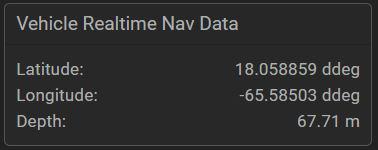
\includegraphics{images/image17.png}

\hypertarget{vehicle-realtime-usbl-data}{%
\subsubsection{Vehicle Realtime USBL
Data}\label{vehicle-realtime-usbl-data}}

\begin{itemize}
\tightlist
\item
  USBL is a method of underwater navigation that uses a transceiver head
  lowered under the ship that communicates with a beacon on the ROV,
  computing the range and angle from the transceiver head to the beacon.
  The software then can determine the position of the beacon on the ROV.
\item
  This is a very accurate form of underwater navigation, but is
  generally not as accurate as the Sprint INS solution.
\end{itemize}

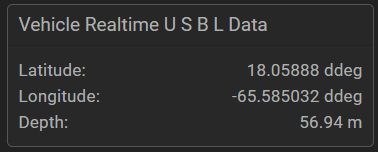
\includegraphics{images/image1.png}

\hypertarget{vehicle-realtime-ctd-data}{%
\subsubsection{Vehicle Realtime CTD
Data}\label{vehicle-realtime-ctd-data}}

\begin{itemize}
\tightlist
\item
  Data from a SBE49 FastCAT CTD
\item
  Realtime measured data:

  \begin{itemize}
  \tightlist
  \item
    Conductivity (uS/cm)
  \item
    Temperature ( C )
  \item
    Pressure (dbar)
  \end{itemize}
\item
  Realtime Derived Variables

  \begin{itemize}
  \tightlist
  \item
    Salinity (ppt)
  \item
    Sound Velocity (m/s)
  \item
    Depth (m)
  \end{itemize}
\end{itemize}

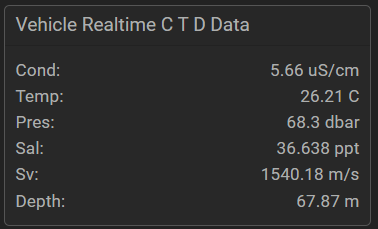
\includegraphics{images/image33.png}

\hypertarget{vehicle-realtime-o2-data}{%
\subsubsection{Vehicle Realtime O2
Data}\label{vehicle-realtime-o2-data}}

Values shown are corrected to account for the effects of salinity and
pressure . Raw values are available in separate data files if needed.

\begin{itemize}
\tightlist
\item
  Aanderaa Oxygen Optode

  \begin{itemize}
  \tightlist
  \item
    Concentration: 196.9 umol
  \item
    Saturation: \%
  \end{itemize}
\end{itemize}

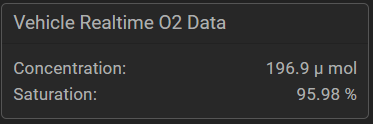
\includegraphics{images/image30.png}

\hypertarget{vehicle-realtime-paro-data}{%
\subsubsection{Vehicle Realtime Paro
Data}\label{vehicle-realtime-paro-data}}

\begin{itemize}
\tightlist
\item
  Paroscientific Digiquartz Depth Sensor (m)
\end{itemize}

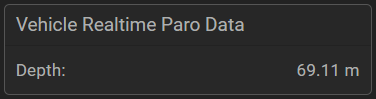
\includegraphics{images/image32.png}

\hypertarget{sealog-in-use}{%
\section{Sealog in Use}\label{sealog-in-use}}

Once event templates are set up for your dive\ldots now it's time to put
the templates in action.

\hypertarget{who-can-use-sealog}{%
\subsection{Who Can Use Sealog?}\label{who-can-use-sealog}}

\begin{itemize}
\tightlist
\item
  Every dive, SOI has a datalogger on watch, who works to track
  information specific to the vessel's need for operation and outreach
  and to ensure specific vehicle milestones are set up for Sealog's
  reporting mechanisms.
\item
  It's up to the science party to provide watchstanders who will log and
  keep track of scientific data logging needs. Generally at least one
  (if not all) watchstanders are in charge of adding events as needed
  during a dive.
\item
  Any scientist onboard the ship who wants to contribute to event
  logging is able to do so.
\end{itemize}

\hypertarget{what-do-we-log}{%
\subsection{What Do We Log?}\label{what-do-we-log}}

\begin{itemize}
\tightlist
\item
  Crewmembers will log Vehicle Events that are critical to Sealog
  operation and reporting mechanisms. We also will log certain
  highlights for our Outreach team. All of our events will be available
  to scientists in the data exports and reports.
\item
  We recommend that Scientists communicate internally about what kinds
  of events should be logged to best serve your needs. Some examples may
  be:

  \begin{itemize}
  \tightlist
  \item
    Wide angle and/or zoom screengrabs of samples prior to sampling.
  \item
    Screengrabs to capture sample storage location.
  \item
    Screengrabs of biological observations.
  \item
    Screengrabs of anthropological observations.
  \end{itemize}
\end{itemize}

\hypertarget{when-do-we-log-events}{%
\subsection{When Do We Log Events?}\label{when-do-we-log-events}}

\begin{itemize}
\tightlist
\item
  Sealog works best when events are logged during an active dive.
\item
  Often scientists will assign certain individuals to be incharge of
  logging in Sealog per watch.
\item
  We can also log Sealog after the fact, but the screen grabs and
  metadata are NOT captured.
\item
  ASNAP is an automatic screengrab that is run at a designated timed
  interval during the dive. The default settings have ASNAP running once
  every 60 seconds, that will take a screengrab of video and metadata,
  so a reasonable log of the dive will exist with minimal science events
  logged.
\end{itemize}

\hypertarget{where-can-we-use-sealog}{%
\subsection{Where Can We Use Sealog?}\label{where-can-we-use-sealog}}

\begin{itemize}
\tightlist
\item
  Currently, Sealog is only available onboard Falkor (too)'s intranet.
\item
  You can log events anywhere on the ship that has internet
  connectivity.
\item
  In the future we hope to provide access to Sealog for scientists
  ashore.
\end{itemize}

\hypertarget{how-should-we-use-sealog}{%
\subsection{How Should We Use Sealog?}\label{how-should-we-use-sealog}}

\begin{itemize}
\tightlist
\item
  We provide the resource and it's up to you as the science party to
  decide your cruise best practices.

  \begin{itemize}
  \tightlist
  \item
    Some examples may include:

    \begin{itemize}
    \tightlist
    \item
      Taking a screengrab prior to any sample.
    \item
      Adding any important information to be noted with each sample such
      as ID or storage location.
    \item
      Log certain observations during a dive like anthropogenic or
      biological.
    \item
      Duplicating key notes into a spreadsheet or logbook.
    \end{itemize}
  \end{itemize}
\end{itemize}

\hypertarget{filtersearching-for-an-event}{%
\section{Filter/Searching for An
Event}\label{filtersearching-for-an-event}}

\begin{itemize}
\item
  On the main screen, the ``Event History'' box has a filter box. It's
  important to note that this will only filter button names and wont
  ``search'' for a keyword in the text or options.
\item
  The example below shows how you can filter your events to show only
  the events that are associated with ``VIDEO LOGGING.''

  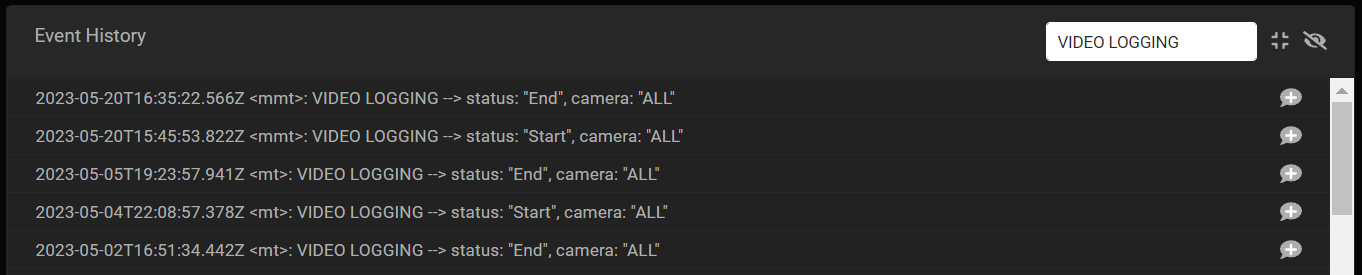
\includegraphics[width=0.7\textwidth,height=\textheight]{images/image3.png}
\item
  To search keywords, navigate to the following location:

  \begin{itemize}
  \tightlist
  \item
    Review Cruises/Dives
  \item
    Select the appropriate year and cruise.
  \item
    Select the dive.
  \item
    Select ``Review''
  \item
    The Event Filter window will appear.

    \begin{itemize}
    \tightlist
    \item
      Event Value: searches only the Event Value (ex. Vehicle, Samples,
      etc).
    \item
      Author: searches for all entries by a certain author.
    \item
      Time: Gives you events within a certain time window.
    \item
      Freeform Text: Searches the ``text'' field present on all events
    \end{itemize}
  \end{itemize}
\end{itemize}

\hypertarget{data-exports}{%
\section{Data Exports}\label{data-exports}}

After every dive, a script is run that will summarize the dive, compile
all of the metadata and send it to the PI-NAS. The following exports are
available after every dive.

\begin{itemize}
\item
  Dive Video

  \begin{itemize}
  \tightlist
  \item
    Science Camera- SCITOO (4K)
  \item
    Situational Camera- SITTOO (4K)
  \item
    HD Quads
  \item
    SD Quads
  \end{itemize}

  File name: \{camera\}\_\{YYYYMMDD\}T\{HHMMSS\}Z.mov
\item
  Images from all of the events, named by camera/date/time of the
  snapshot.
\item
  Dive Summary Report PDF (explained in detail below).
\item
  Vehicle Summary Report PDF (explained in detail below).
\item
  Sealog Export (CSV, JSON)
\item
  All the information from the dive, every event with associated
  metadata included.
\item
  Aux Data Export (JSON)
\item
  Auxiliary data sensors during the dive such as CTD, O2, High Temp
  probe, etc.
\item
  Event Only Export (CSV, JSON)
\item
  Export of events and their options and comments.
\item
  Event Templates (JSON)
\item
  Sealog configuration file for the dive, grabbing all of the event
  templates configured.
\item
  Lowering Record (JSON)
\item
  Dive number, location, and summary.
\end{itemize}

\hypertarget{dive-reports}{%
\section{Dive Reports}\label{dive-reports}}

\hypertarget{dive-summary-report}{%
\subsection{Dive Summary Report}\label{dive-summary-report}}

Each dive, a summary report gets produced which includes the following
information and graphics:

\begin{itemize}
\item
  Dive Overview

  Includes dive number, location, and summary.
\end{itemize}

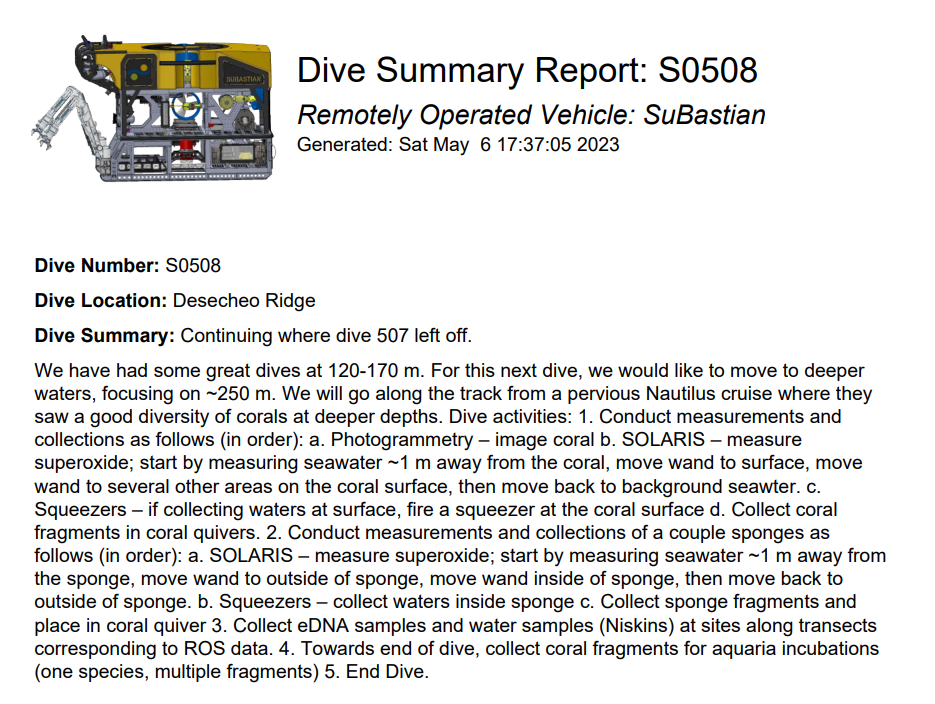
\includegraphics{images/image6.png}

\begin{itemize}
\item
  Dive Timeline

  Includes key dive milestone timelines, max depth, and number of
  samples collected
\end{itemize}

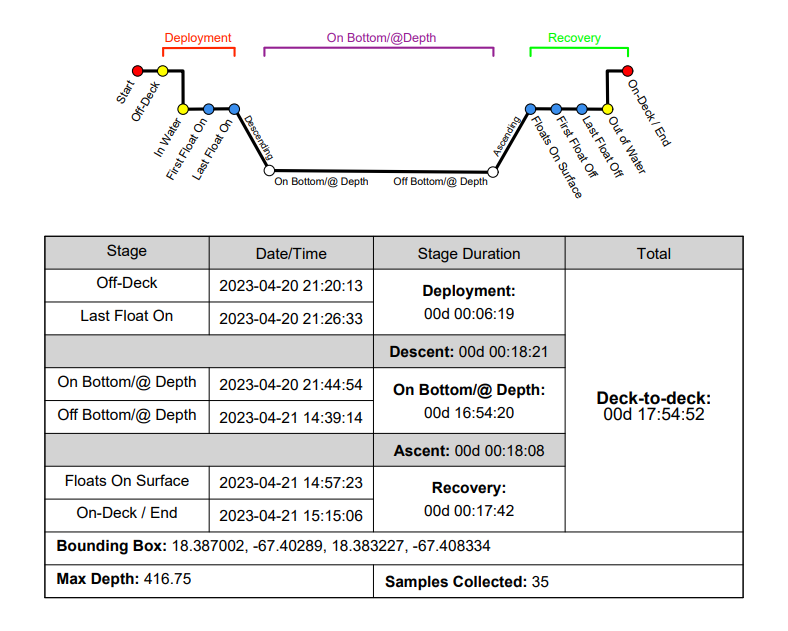
\includegraphics{images/image12.png}

\begin{itemize}
\item
  Dive Track

  Visual display of the ROV's track throughout the dive.
\end{itemize}

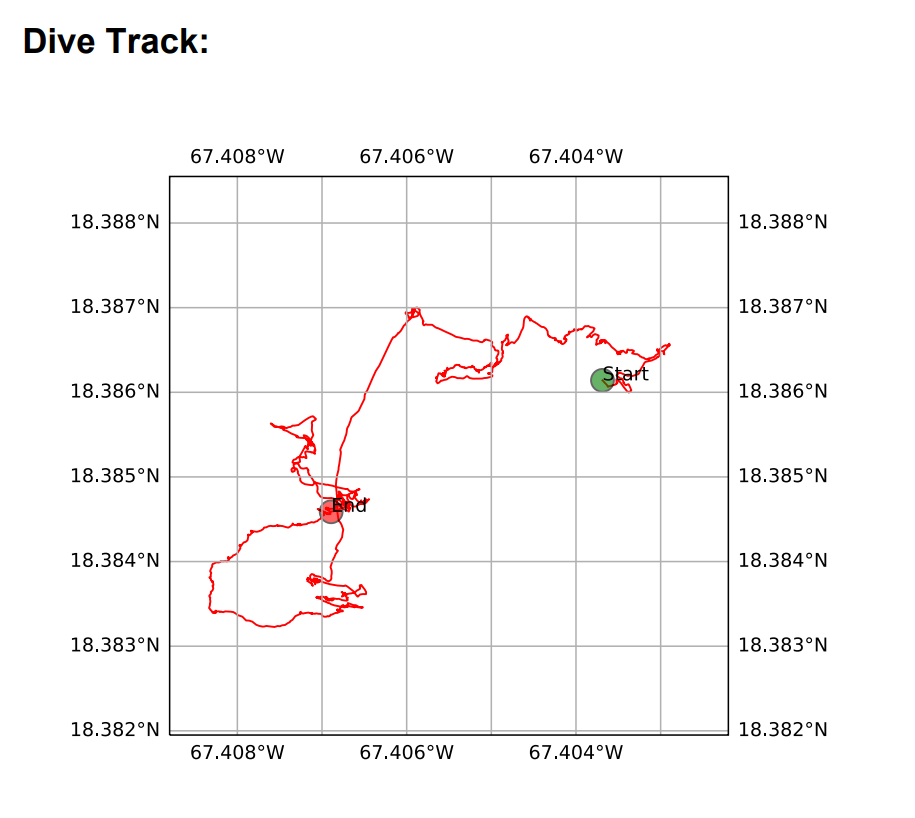
\includegraphics{images/image25.png}

\begin{itemize}
\item
  Depth Profile

\begin{verbatim}
  Comparison of all the depth sensor’s dive profile
\end{verbatim}
\end{itemize}

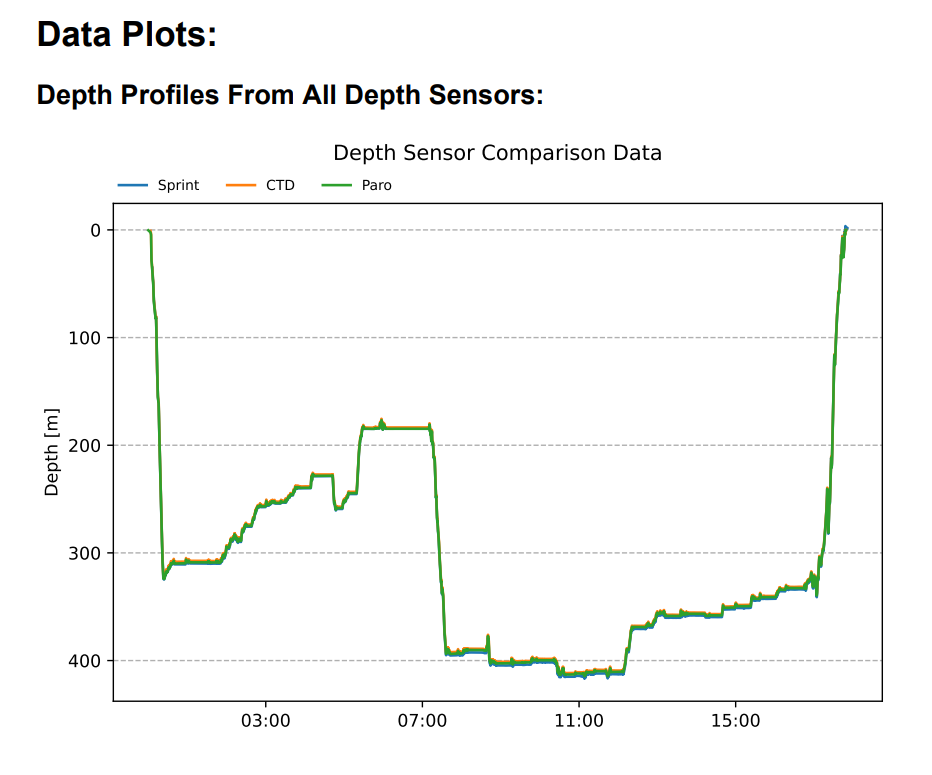
\includegraphics{images/image13.png}

\begin{itemize}
\item
  CTD Profile

  Profiles of conductivity, temperature, salinity and depth for the
  descents and ascents.
\end{itemize}

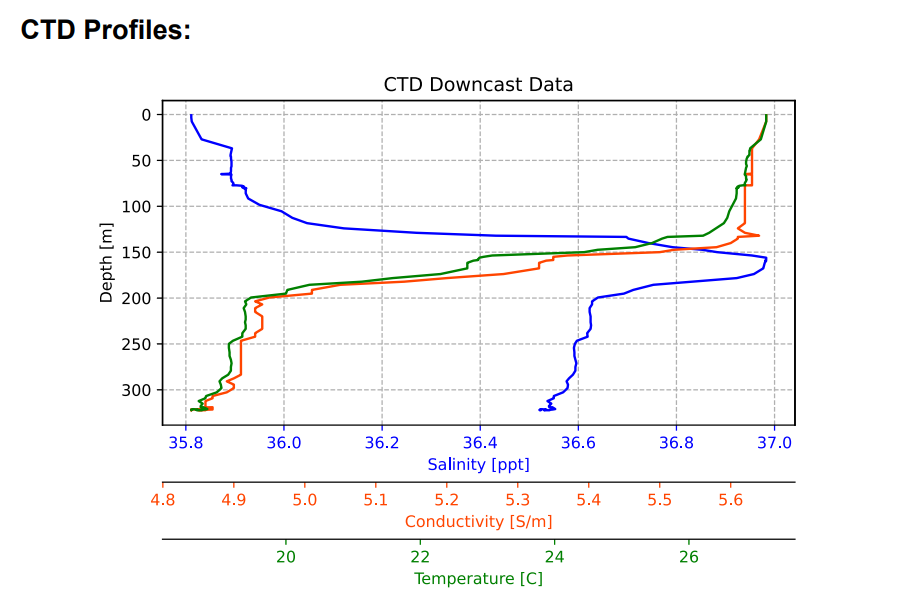
\includegraphics{images/image34.png}

\begin{itemize}
\item
  Problems

\begin{verbatim}
  Any problems (either vehicle or science related) for the dive. 
\end{verbatim}
\end{itemize}


\includegraphics{images/image24.png}

\begin{itemize}
\item
  Events Breakdown Table

  Count of all the Event Value's recorded on the dive
\end{itemize}

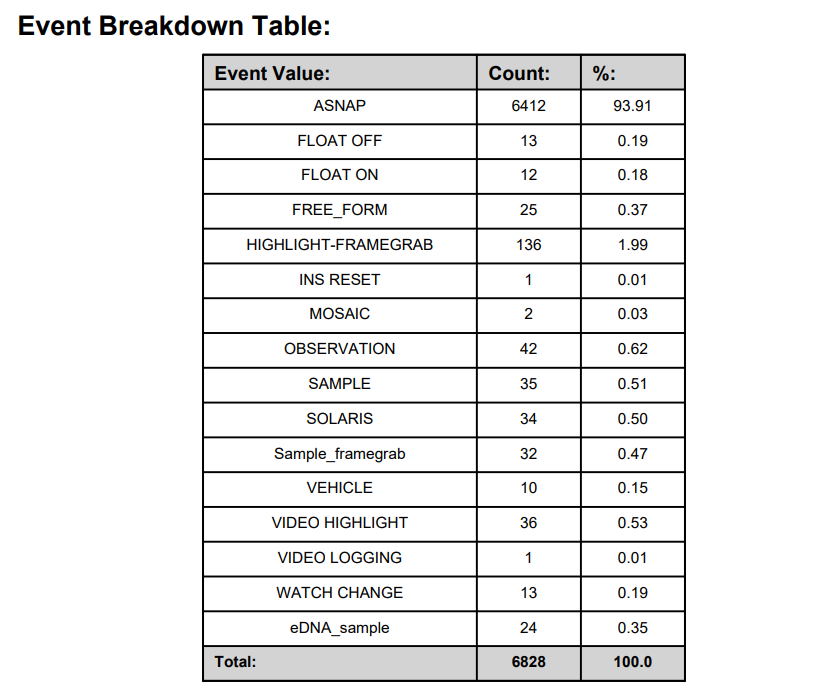
\includegraphics{images/image31.png}

\begin{itemize}
\item
  Event Value Table

\begin{verbatim}
  Each Event Value gets its own table with metadata for each individual event. 
\end{verbatim}
\end{itemize}

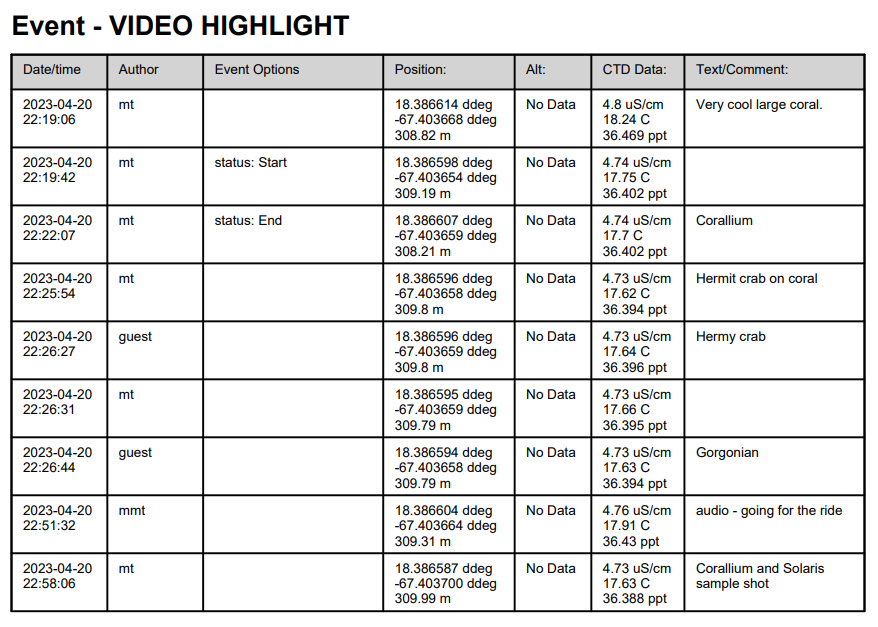
\includegraphics{images/image27.png}

\hypertarget{vehicle-summary-report}{%
\subsection{Vehicle Summary Report}\label{vehicle-summary-report}}

This report is meant to be a summary of events that the ROV pilots can
use to keep track of vehicle information. Most of the data here is more
extensively covered in the Dive Summary Report. Vehicle Summary Report
includes:

\begin{itemize}
\tightlist
\item
  Dive Timeline
\item
  Dive Track
\item
  Depth Profile
\item
  Depth Sensor Comparison Plot
\item
  ROV Compensator Pressure Data
\item
  CTD Profiles
\item
  Problems
\item
  Watch Change Times
\end{itemize}

\hypertarget{frequently-asked-questions}{%
\section{Frequently Asked Questions}\label{frequently-asked-questions}}

\begin{itemize}
\item
  Is it possible to log an event in the past?

  Yes, at the bottom of each event template entry, there is an option
  for ``Custom Time (UTC).'' This can be used to adjust the time of the
  event, however Sealog will not grab past metadata for this entry.
\item
  Which ROV Depth value is most accurate?

  Accuracy for depth is very much dependent on several factors (sensor
  calibration, depth, latitude, etc) your best option is to ask the MT's
  on your cruise.
\item
  There are multiple positions in the metadata, which ones should I
  use?''

  USBL position is solely based on the USBL underwater tracking of the
  vehicle. The Realtime Nav Data is SuBastian's INS, which takes into
  account several inputs to make an educated calculation on position. In
  general, Realtime Nav Data is the position you should be using, but
  always ask the MT's on your cruise.
\item
  Can I delete an event?

  Only system administrators have the ability to delete an event, but
  you can ask an MT to delete it for you if needed.
\item
  Can I edit a past event?

  You cannot edit a past event, but you can add a ``comment'' to the
  event where you can correct or add more information.
\item
  When I search for a known event, nothing is shown.

  Great Question! We are still working on this one :)
\item
  Can I review the dive after it is over?

  Yes, while on the ship you can review the dive. All of the data during
  the dive is being transferred to the PI-NAS, which you'll have access
  to throughout the cruise. Shortly after the end of a dive, the dive
  summary and screengrabs will be available on the PI-Nas.
\item
  Can I replay a dive?

  Under Review Cruises/Dives, after you've navigated to the correct
  year, cruiseID and dive number, you can select ``Replay'' which will
  allow you to step through every event logged during that dive.
\item
  Am I able to login to Salog after I am off the ship?

  Currently this is not available, however all data associated with
  Sealog is found in your Cruise Data Folder under each dive.
\item
  What if I forgot to screen grab an event?

  Sealog has a feature called ``ASNAP'' that takes a screengrab on a
  designated timed interval. The default is set to 1 per minute, but
  depending on your needs, you can make this more or less frequent.
  Speak to the Marine Technicians about changing your ASNAP interval.
\item
  Can we change templates after initial configuration?

  Yes of course, you can change templates to better fit your needs
  anytime, but it's recommended that you spend time prior to the first
  dive to get the dive templates to fit your needs. Certain templates
  (like sampling) need to be approved by Marine Technicians.
\end{itemize}

\appendix
\addcontentsline{toc}{part}{Appendices}

\hypertarget{appendix}{%
\chapter{Appendix}\label{appendix}}

\hypertarget{references}{%
\chapter*{References}\label{references}}
\addcontentsline{toc}{chapter}{References}

\markboth{References}{References}

\hypertarget{refs}{}
\begin{CSLReferences}{0}{0}
\end{CSLReferences}



\end{document}
